Here, we provide background on energy harvesting systems and the intermittent software execution model. We then discuss the key limitations of existing task-based execution models for intermittent computing that \sys addresses.

\subsection{Energy Harvesting Systems}
\label{sec:background_harvesting}

Energy harvesting devices operate using energy extracted from their environment, from sources such as radio waves and solar energy. Energy-harvesting devices do not use a tethered power supply or battery and instead, typically collect energy into a (super-)capacitor, operate when sufficient energy has accumulated, and upon depleting the stored energy, turn off and wait to collect more energy.
%
%Batteryless operation has a number of important advantages, making intermittent computing an important research domain. Supplying power to billions~\cite{gartner_iot} of embedded computers using batteries is not sustainable. The European Commission estimates that more than 160 kilotons of consumer batteries enter the European Union annually~\cite{eu_batteries_2016}. Batteries are an environmental risk, are fragile, are limited in their number of charge/discharge cycles, and may require costly physical maintenance that is difficult or impossible deployed (e.g. in space~\cite{kicksat}). By contrast, super-capacitors are durable, promising millions of charge/discharge cycles~\cite[Sec. I]{ongaro_pwre_2012}. The main limitation in moving to capacitor-based energy storage is that capacitor energy density---and consequently operating discharge time---is orders of magnitude less than a battery. 
%
%Given current technology development, battery-less systems are best suited for very long-term sensing and monitoring where access to recharge is either prohibitive or impossible. These include battery-less image capture and processing~\cite{naderiparizi_rfid_2015}, animal monitoring~\cite{thomas_jbcs_2012} or implantable~\cite{rodriguez_tbcs_2015} and digestible~\cite{nadeau_naturebio_2017} sensors.
%
Many platforms enable intermittent, battery-less energy harvesting-based computation. For instance, computational RFIDs---open-source TI MSP430-based~\cite{wolverine} WISP~\cite{wisp5} (with its variants such as WISPCam~\cite{naderiparizi_rfid_2015}, NFC-WISP~\cite{zhao_rfid_2015} or NeuralWISP~\cite{holleman_biocas_2008}), Moo~\cite{moo}, and commercial ones such as~\cite{medusa_farsens_2017}. Other intermittently-powered platforms include ambient backscatter tag~\cite{liu_sigcomm_2013,parks_sigcomm_2014} or battery-less phone~\cite{talla_imwut_2017}. 

%In all of the above, the main source of energy harvested is the electromagnetic radiation in the radio frequency range (ambient transmitters such as high power TV transmitters~\cite{liu_sigcomm_2013} or dedicated RFID antenna~\cite{wisp5,moo,talla_imwut_2017,medusa_farsens_2017,holleman_biocas_2008,naderiparizi_rfid_2015}). Naturally, other forms of energy harvesting sources exist, including temperature gradient, (micro-)motions, light/sun radiation, vibrations, and body fluid flow (blood, gastric acid). Several recent surveys discussing energy harvesting, low-power, embedded systems and intermittent computing at a high level~\cite{paradiso_pvc_2005,soyata_csm_2016,prasad_comst_2014,ku_cst_2016,lucia_snapl_2017}.

\subsection{Intermittent Computing}
\label{sec:background_consistency}

Energy-harvesting devices execute software according to the {\em intermittent execution model}~\cite{dino,chain,alpaca,ratchet}.
%
%Physically, a device charges until a threshold, operates briefly until its energy is depleted, shuts down recharges, and repeats the cycle.
%
Software running on the device executes {\em intermittently} because energy is only available between when the capacitor reaches its threshold and when it is depleted. An intermittent execution is composed of operating periods interspersed with power failures. The frequency of power failures in an intermittent execution depends on the size of the device's energy storage buffer: a larger buffer allows longer operating periods. Energy-harvesters provide input power that is orders of magnitude less than a device's operating power, making recharging negligible during operation.

Software has different behavior when executed intermittently than when executed with continuous power. Each power failure clears volatile memory (registers, stack, and global variables). Non-volatile memory (e.g., FRAM) persists across power failures. On a power failure, control flows back to a prior point in the execution. By default, after a power failure control flows to the beginning of {\tt main()}. Early work on intermittent computing preserved intermittent progress by periodically capturing and restoring to a non-volatile checkpoint of the volatile execution context, i.e., registers and stack~\cite{mementos,quickrecall}, sometimes using hardware support~\cite{mementos,mottola2017harvos,hibernusplusplus,hibernus,idetic}. 

\begin{figure}
	\centering
	\subfloat[Simplified C code snippet of a CRC calculation from~\cite{hicks_mibench2_2016}: per-byte message division by a polynomial; \texttt{NV} denotes non-volatile variable declaration]{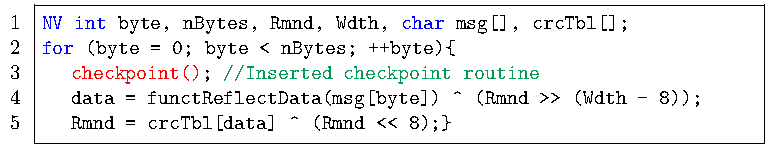
\includegraphics[width=\columnwidth]{figures/crc_example}\label{fig:crc_example}}\\
	\subfloat[Consecutive execution steps of the loop body in the snippet above: non-volatile checkpointing did not guarantee data consistency as data has been manipulated (line 10) with stale reminder (line 3)]{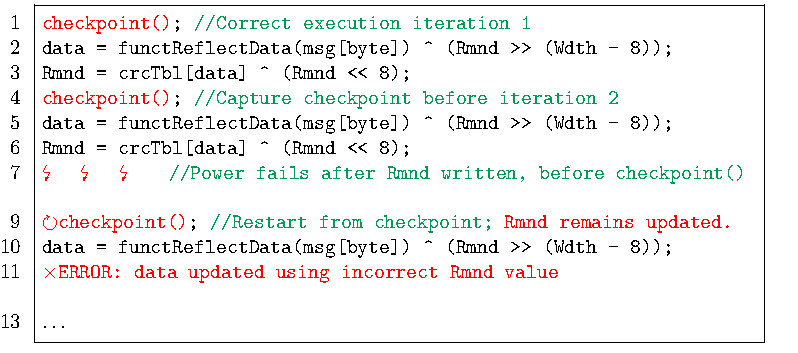
\includegraphics[width=\columnwidth]{figures/crc_example_war}\label{fig:crc_example_war}}
	\caption{Code example demonstrating effect of write after read on volatile memory checkpointing.}
	\label{fig:code_demo_incosistency}
\end{figure}

Checkpoints of volatile state preserve intermittent progress, but do not ensure data consistency~\cite{dino,chain,ratchet}. Data may become inconsistent if an attempt to execute some computation {\em writes} to a non-volatile variable, then power fails, then a second attempt to re-execute the same computation incorrectly {\em reads} the value written in the first attempt, rather than the variable's original value.  The situation occurs when code includes a write after read (WAR) dependence between operations that manipulate non-volatile variables~\cite{ratchet,dino,alpaca}.

Figure~\ref{fig:code_demo_incosistency} illustrates how state can become inconsistent in an intermittent execution using the cyclic redundancy check (CRC) code from MIBench~\cite{hicks_mibench2_2016}. The code computes the CRC for an $\texttt{nBytes}$ byte message $\texttt{msg}$ with remainder $\texttt{Rmnd}$. Even with the checkpoint at line 3 in Fig.~\ref{fig:crc_example}, the code may compute  $\texttt{data}$ incorrectly because of a WAR dependence between the read of $\texttt{Rmnd}$ on line 4 and the write of $\texttt{Rmnd}$ on line 5. Figure~\ref{fig:crc_example_war} shows an execution of the code in which power fails during the second loop iteration. The problem arises because line 6 of the execution writes $\texttt{Rmnd}$ in the second iteration, but power fails before capturing the next checkpoint. After restarting from the checkpoint, the update to $\texttt{data}$ at line 10 reads the value of $\texttt{Rmnd}$ that was updated before the power failure, producing an incorrect result.

As the figure illustrates, checkpoint-based systems risk violating the volatile and non-volatile memory consistency~\cite{dino}. To maintain consistency, versioning systems~\cite{dino,ratchet} {\em version} a subset of non-volatile variables with the checkpointed execution context. Task-based systems~\cite{chain,alpaca}, which we focus on this work and discuss in detail next, ensure state consistency by using programmer, compiler, and runtime support.

\subsection{Task-based Intermittent Computing}
\label{section:background_task_computing}

Task-based intermittent execution models~\cite{dino,chain,alpaca} ask the programmer to decompose their program into a collection tasks. A task is a function with no caller that contains arbitrary computation, sensing, and communication. A programmer describes the sequence in which tasks may execute, creating a task graph. The flow of control from task to task happens at programmer demarcated points and may conditionally depend on program values. Task-based programming abstractions guarantee that tasks exhibit behavior as though they executed {\em atomically}, regardless of arbitrary power failures. Task-based runtime systems tolerate failures by repeatedly attempting to execute a task until it completes. Task-based runtime systems ensure task-atomic semantics by ensuring that repeated task executions are idempotent (i.e., have the same effect when repeatedly executed). The key to idempotence is ensuring that updates to non-volatile state made by an interrupted, partial execution of a task are never visible to a subsequent (potentially completing) re-execution of the task.  

There are several run time strategies to ensuring task idempotence. One approach, utilized by Alpaca~\cite{alpaca}, is to identify non-volatile data involved in WAR dependences in a task (like DINO~\cite{dino} and Ratchet~\cite{ratchet} did for checkpoints), execute the task using buffered copies of those data, and commit the buffered copies before completing the task. Another strategy is to statically create multiple versions of non-volatile data shared by tasks and ensure by construction that no task reads and writes the same non-volatile memory location~\cite{chain}. Regardless of the idempotence strategy, the key to task-based execution is that fixed, statically-defined tasks execute as though atomic, completing after zero or more attempts. 

\begin{table}
	\centering
	\footnotesize
	\begin{tabular}{|c|c|}
		\hline
		Model & Data Copied to/from NVRAM \\
		\hline\hline
		Mementos~\cite{mementos}                             & Reg. + Stack     \\
		DINO~\cite{dino}                                     & Reg. + WAR variables \\
		Chain~\cite{chain}                                   & PC   + Channel data\\
		Alpaca~\cite{alpaca}                                 & PC   + WAR variables \\
		Ratchet~\cite{ratchet}, Clank~\cite{hicks_isca_2017} & Reg. (requires NV main memory) \\
		\hline
	\end{tabular}
	\caption{Memory consistency enforcement overheads of various intermittent execution models. \emph{Reg.} includes the entire register file, \emph{PC} is the program counter, \emph{Channel data} are variables explicitly task-shared by the programmer, and \emph{WAR variables} are variables involved in WAR dependences (\emph{NV}: non-volatile).}
	\label{table:chechpoint_comparison}
\end{table}

\subsubsection{Costs of Task-based Models}

Task-based intermittent execution models ensure that programs execute correctly despite arbitrary power failures and in doing so, incur several costs that are the motivation for \sys. 

\noindent \textbf{Memory Consistency Enforcement Overhead:} Intermittent execution models incur an overhead because they must checkpoint data~\cite{dino,ratchet,quickrecall,mementos}, manage channels~\cite{chain}, or privatize and commit data~\cite{alpaca}. Table~\ref{table:chechpoint_comparison} compares the overheads for several recent intermittent execution models (generalizing discussion from~\cite[Sec. 2.4]{alpaca}.) The mechanism responsible for the overhead of each model varies, but all the bulk of overhead in all models is a manipulating non-volatile memory. Checkpointing moves volatile memory and registers to and from non-volatile memory, channel accesses directly manipulate non-volatile data~\cite{chain}, privatization copies data from and commits data to non-volatile memory~\cite{alpaca}, and idempotence solutions~\cite{ratchet} require all of memory to be non-volatile.  

\begin{figure}
	\centering
	\subfloat[Energy cost of \emph{write} operation]{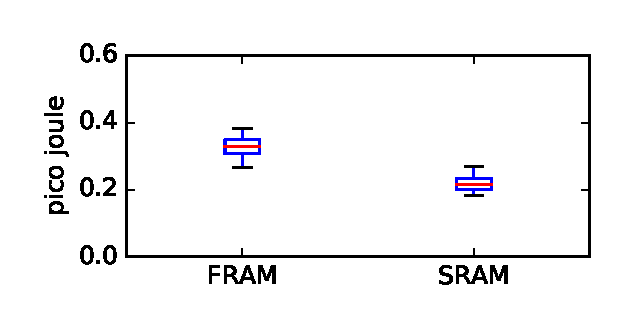
\includegraphics[width=0.49\columnwidth]{figures/fram_write.eps}}
	\subfloat[Energy cost of \emph{read} operation]{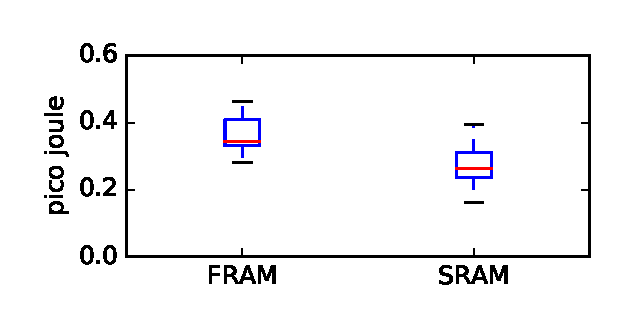
\includegraphics[width=0.49\columnwidth]{figures/fram_read.eps}}
	\caption{Energy cost of accessing volatile (SRAM)/non-volatile (FRAM) memory during write (left) and read (right) operation.}
	\label{fig:framEnergy}
\end{figure}

To concretely understand the cost of these manipulations of non-volatile memory, we directly measured the energy consumption of volatile (SRAM) and non-volatile (FRAM) memory operations for the MSP430FR5969~\cite{msp430datasheet} microcontroller. We used EDB~\cite{edb} to monitor the voltage drop on an energy buffering capacitor that powers the device across 1600 read and write accesses to each type of memory, randomizing locations to avoid caching effects. Figure~\ref{fig:framEnergy} summarizes these measurements, illustrating that a non-volatile memory access consumes around 1.5 times as much energy as a volatile memory access in this device. In an intermittently-powered device, the increased energy corresponds to decreased run time between power failures. The overheads imposed by relying on non-volatile memory motivate \sys, which uses memory virtualization to operate primarily using volatile SRAM.

The above result reassures the intuitive observation that a decrease of checkpoint frequency (CP) decreases the energy cost associated with each state preservation method and reduces operation cost which in most simplistic terms is defined as $\mathcal{O}(\text{CP})+\mathcal{O}(\text{PL})$, where PL is the cost of program execution without checkpointing. On the other hand, this increases task/checkpoint re-execution time. The ideal solution is a runtime that \emph{adaptively} changes task size during runtime, which however exposes a second problem.

\begin{table}
	\centering
	\footnotesize
	\begin{tabular}{|c|c|}
		\hline
		Platform name & Storage capacitor size \\
		\hline \hline
		%Moo~\cite{moo} & 0.1\,F \\
		WISPCam~\cite{naderiparizi_rfid_2015} & 6.08\,mF \\ %tested [11.24, 17.45, 21.98]\,mF
		%NFC-WISP~\cite{zhao_rfid_2015} & 300\,$\mu$F \\
		NeuralWISP~\cite{holleman_biocas_2008} & 100\,$\mu$F \\
		WISP~\cite{wisp5} & 47\,$\mu$F \\
		{\em BioImpedance} sensor~\cite{rodriguez_tbcs_2015} & 20\,$\mu$F \\
		{\em Ingestible} sensor~\cite{nadeau_naturebio_2017} & 220\,$\mu$F\\
		\hline
	\end{tabular} 
	\caption{Comparison of {\em default} energy storage sizes for example battery-less platforms. Observe a huge variation in storage capacity.}
	%We note that values for other representative platforms~\cite{medusa_farsens_2017,talla_imwut_2017,liu_sigcomm_2013,parks_sigcomm_2014} were not reported in their respective papers.
	\label{table:capacitor}
\end{table}

\noindent \textbf{Fixed-size Tasks are Inflexible and Inefficient:} A programmer must write each task with statically defined boundaries, which makes statically-sized tasks inflexible and non-portable. The programmer must ensure statically that a task's energy requirements match the device's energy storage capacity. If a programmer writes a task that consumes more energy than the device can buffer, the task will never be able to complete using the buffered energy. The consequence of such tasks is a non-progressing program that repeatedly attempts to re-execute the task of excess energy cost. If a programmer writes a program that consumes less energy than the device can buffer, the system may operate inefficiently. When a task and its successor both complete, the two tasks were interrupted by a task boundary that preserves progress and state (i.e., checkpoint or commit).  If the two tasks were not also interleaved by a power failure, then the computation done to preserve state was {\em unnecessary}, only incurring an overhead on the tasks' executions. Avoiding excessively costly, non-terminating tasks and short, high-overhead tasks is a programming challenge, given fixed hardware with a fixed energy buffering capacity that might be \emph{different} for each transiently-powered device (see Table~\ref{table:capacitor}). Such tasks also make it extremely difficult to {\em port} code from  one device to another. A task that is excessively costly on a device with a small energy buffer may become a short, high-overhead task on a device with a larger energy buffer and vice versa. The key problem is that the programmer writes tasks statically for an energy buffer of a fixed size. \sys's {\em task coalescing} mechanism, which we will describe in Section~\ref{sec:task_coalescing}, is motivated by the observation that systems with statically-defined tasks may be inflexible and inefficient. 

\subsection{Hardware Assumptions}
\label{sec:background_hardware}

\sys is designed for the demands of existing and future energy-harvesting platforms based around general purpose, commodity computing components~\cite{wisp,msp430datasheet}. We assume a device with a memory system that has fast, byte-addressable volatile and non-volatile memory; in particular, our target platform~\cite{wisp} is equipped with a mixture of SRAM and FRAM. Our implementation leverages hardware support for fast, bulk-copying between memories via DMA~\cite{msp430datasheet}. We do not require a particular non-volatile memory technology, nor do we require architectural additions commodity processors~\cite{su_date_2017,ratchet,quickrecall,nvp}. \sys supports I/O behavior similar to recent intermittent execution models~\cite{alpaca,chain}, allowing safe, synchronous I/O and unsafe, asynchronous I/O.